% questions.tex —— 1958 年·华东卷（上海、福建） · 题目内容片段（无答案）
% 由 tools/generate_projects.py 依来源总账自 1958/1958_华东(上海,福建)_数学真题_试题.md 生成，勿手改（改源 MD 后重跑）


\begin{question}
\gkti{1}设方程 $x^{2}-(m-2)x-(m-6)=0$ 有二个不相等实根，决定 $m$ 范围。

\end{question}
\begin{question}
\gkti{2}解方程组：

\nopagebreak[4]
\[
\begin{cases}
\dfrac12\lg x+\dfrac12\lg y-\lg(4-\sqrt{x})=0,\\[2pt]
\left(25^{\sqrt{x}}\right)^{\sqrt{y}}-125\times5^{\sqrt{y}}=0.
\end{cases}
\]

\end{question}
\begin{question}
\gkti{3}一九五七年我国钢产量约 500 万吨，同年英国钢产量 2000 万吨，根据英国每年平均增长率为 4.24\%，如果我国准备四年在钢的产量方面赶上英国，问每年平均增产的百分率是多少（精确到 0.01）？

\end{question}
\begin{question}
\gkti{4}设有函数 $y=ax^{2}+bx+c$，当 $x=1$ 时，$y=-1$；当 $x=2$ 时，$y=1$；又当 $x=-2$ 时，$y=17$。

（1） 决定这函数式；

（2） 这函数有无极大值或极小值？如果有，其值是什么？

（3） 当 $x$ 是什么值时，这函数值为 $0$？

（4） 作出函数图像。

\begin{gktip}
\textbf{题号说明}：原卷本题四问以 A)、B)、C)、D) 编号，本转录按体例统一为（1）、（2）、（3）、（4），内容不变。
\end{gktip}

\end{question}
\begin{question}
\gkti{5}河的对岸有 $A,B$ 两点，要在这边测量 $A,B$ 间的距离，应该怎样测量？试拟出一种方法来进行说明，并写出表达距离的式子（即把能测得的角和能量得的距离的数值表示 $A,B$ 间的距离）。

\Needspace{0.4\textheight}
\end{question}
\begin{question}
\gkti{6}两平行线 $L_1$ 与 $L_2$ 分别和已知圆相切于 $A$ 与 $B$ 点，作已知圆的任一切线 $L_3$，与 $L_1,L_2$ 分别相交于 $C$ 与 $D$ 点，证明乘积 $AC\cdot BD$ 是常量。
\nopagebreak[4]
\begin{center}% 1958 年华东(上海,福建)卷第 6 题：两条水平平行切线 L1（上）、L2（下）切圆 O 于 A、B，第三条切线 L3 交 L1 于 C、交 L2 于 D（按源卷布局；L3 与圆的切点原卷未标字母，故不标）
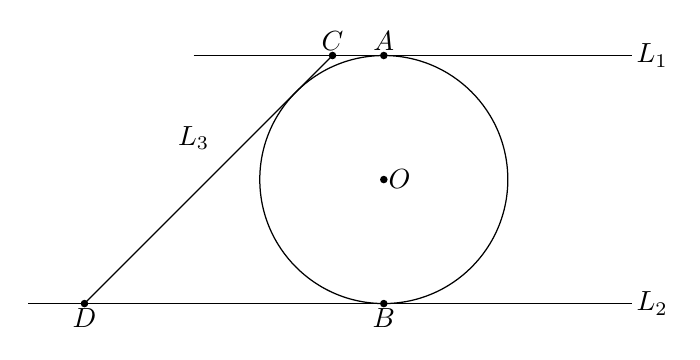
\begin{tikzpicture}[scale=1.05, line width=0.45pt,
  every node/.style={inner sep=1.5pt}]
  \coordinate (O) at (0,0);
  \coordinate (A) at (0,1.5);
  \coordinate (B) at (0,-1.5);
  \coordinate (C) at (-0.62,1.5);
  \coordinate (D) at (-3.62,-1.5);
  \draw (-2.3,1.5) -- (3,1.5);
  \draw (-4.3,-1.5) -- (3,-1.5);
  \draw (O) circle (1.5);
  \draw (C) -- (D);
  \fill (A) circle (1.3pt);
  \fill (B) circle (1.3pt);
  \fill (C) circle (1.3pt);
  \fill (D) circle (1.3pt);
  \fill (O) circle (1.3pt);
  \node[anchor=south] at (A) {$A$};
  \node[anchor=north] at (B) {$B$};
  \node[anchor=south] at (C) {$C$};
  \node[anchor=north] at (D) {$D$};
  \node[anchor=west] at (O) {$O$};
  \node[anchor=west] at (3,1.5) {$L_1$};
  \node[anchor=west] at (3,-1.5) {$L_2$};
  \node at (-2.3,0.5) {$L_3$};
\end{tikzpicture}
\end{center}
\nopagebreak[4]
\end{question}
\begin{question}
\gkti{7}设平面 $S$ 上有一直角三角形 $ABC$，已知一个直角边长为 18 分米，在平面 $S$ 外取一点 $P$，使它与 $A,B,C$ 三点等距离，且设从 $P$ 点到平面 $S$ 的距离为 40 分米，求 $P$ 点到另一直角边的距离。

\end{question}